\chapter{Motor-Encoder}

The TI project recommends using this motor-encoder:

\url{https://www.sparkfun.com/products/13260}

While this motor-encoder kit can be made to work, a better solution was found on eBay:

\begin{figure}[h]
	\centering
    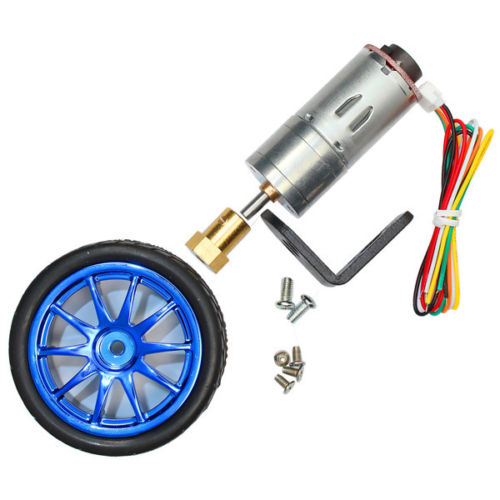
\includegraphics[width=0.5\textwidth]{photos/s-l500.jpg}
	\centering\bfseries
	\caption{eBay Motor-encoder}
\end{figure}

The eBay motor-encoder is a nicely constructed geared DC motor and it has an integrated electronic Quadrature Encoder using Hall-Effect devices.

Also includes is a sturdy mounting bracket, a wired connector, and a brass bushing with matching wheel.  For the purposes of using this in a mobile robot this is very good indeed!

The seller of this motor-encoder was ``kanzezol'' as of December 2016.  This seller also has what appears to be a variant motor-encoder which is less expensive, but it does not include the mounting hardware and wheel.

\section{Quadrature Encoder}

\begin{figure}[h]
	\centering
    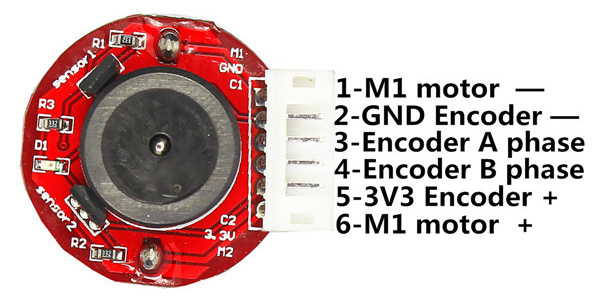
\includegraphics[width=0.5\textwidth]{photos/encoder-close-view.jpg}
	\centering\bfseries
	\caption{The Integrated Quadrature Encoder}
\end{figure}

The suggested DC motor includes an integrated "Quadrature Encoder".  The Quadrature Encoder consists of two Hall-Effect sensors and a rotating magnet attached to the motor shaft.  The rotating magnet has areas of alternating north and south poles.  Thus as the motor shaft turns, the Hall-Effect sensors output a series of pulses with frequency proportional to the rotation velocity "Revolutions Per Minute" (RPM).

Since there are two Hall-Effect sensors, there are two separate pulse outputs.  The Sensors are arranged in physical locations around the rotating magnet such that the two pulse trains overlap.  They overlap with a phase difference of approximately 90 degrees, thus the term "quadrature" is used, however, in practice a precise 90 degree offset does not appear to be critical.

The overlapping pulses allow the sensing of rotational direction, since one sensor will fire first in one direction, and the other sensor will fire first in the opposite direction.  Direction reversal was not included in this project and the feature was not used.

The encoder requires a 3.3 Volt power source.

The 3.3 Volt bias source for the encoder was found to be somewhat critical.  This bias supply could probably be sourced from the BBG, however, this was not attempted.